\documentclass[english,11pt,a4paper]{article}
\usepackage[T1]{fontenc}
\usepackage{graphicx}
\usepackage{mathtools}
\usepackage{amssymb}
\usepackage{amsthm}
\usepackage{thmtools}
\usepackage{xcolor}
\usepackage{nameref}
\usepackage[brazil]{babel}
\usepackage{authblk}
\usepackage{fourier}
\usepackage{indentfirst}
\usepackage{float}
\usepackage{subcaption}
\usepackage[colorlinks, urlcolor=blue]{hyperref}
\title{Introdução à Neurociência Computacional\\Lista de Exercícios 2}
\author{Paulo R. Sturion}
\begin{document}
	\maketitle
	
	\noindent Todos os códigos escritos para produzir os resultados dos exercícios a seguir estão disponibilizados de forma clara e organizada no repositório Github:
	
	\begin{center}
		\noindent \href{https://github.com/prsturion/intro-computational-neurosciene.git}{https://github.com/prsturion/intro-computational-neuroscience.git} \newline
	\end{center}
	
	\noindent \textbf{Questão 1.} Implemente um programa para a solução do sistema de quatro equações (1)--(4) (Modelo de Hodgkin-Huxley). Use como método numérico o método de Euler com passo de integração igual a 0,001 ms. Um valor pequeno de $\Delta t$ é necessário para dar estabilidade numérica à simulação. As quatro variáveis ($V, n, m, h$) devem ser atualizadas a cada passo de simulação, pois elas dependem umas das outras (veja o Apêndice desta lista). Faça seu programa de maneira que a densidade de corrente injetada seja um pulso de amplitude $J$ aplicado no instante inicial $t_i$ e desligado no instante final $t_f$. Faça o programa de tal forma que você possa escolher os valores de $J, t_i$ e $t_f$. Faça com que seu programa dê como respostas os gráficos de $V \times t$, $n \times t$, $m \times t$, $h \times t$ e $J \times t$ de maneira que esses gráficos fiquem juntos; por exemplo, $V \times t$ em um gráfico, as três variáveis de \textit{gating} em outro gráfico, e $J \times t$ em um terceiro gráfico, com os três gráficos alinhados verticalmente. Isso permite a observação e análise das quatro variáveis do modelo de forma conjunta. Tome cuidado na hora de calcular as funções $\alpha_i(V)$ e $\beta_i(V)$, $i = n, m, h$, pois em alguns casos, dependendo do valor de $V$, o valor da função é do tipo ``0/0''. Para evitar isso, use a regra de L'Hôpital: se $f(a) = g(a) = 0$, então
	
	\[
	\lim_{x \to a} \frac{f(x)}{g(x)} = \lim_{x \to a} \frac{f'(x)}{g'(x)}.
	\]
	
	\noindent Inicialmente, faça $J = 0$ e rode seu programa por 30 ms e verifique se a voltagem $V$ se estabiliza em torno de zero. Explique o comportamento observado de $V(t)$ em termos das variáveis de \textit{gating} $n(t), m(t)$ e $h(t)$.
	\\\\
	
	\noindent \textbf{Resposta:} Os gráficos obtidos para os parâmetros dados no enunciado da questão estão exibidos na figura \ref{fig1}.
	
	\begin{figure}[H]
		\centering
		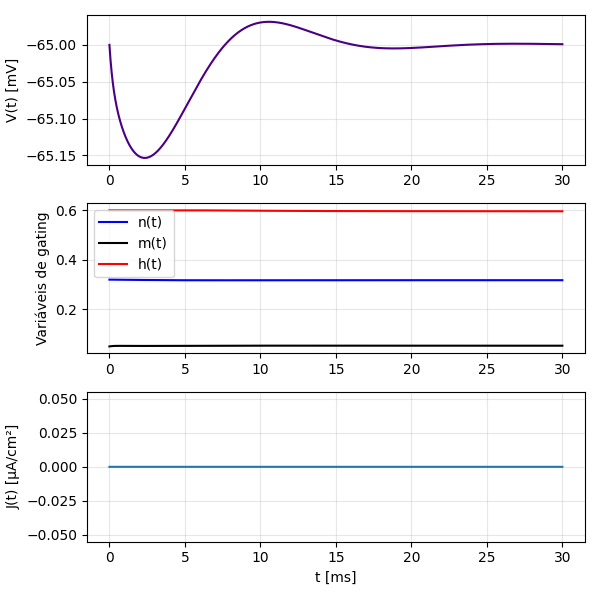
\includegraphics[width=8.5cm]{../figures/ex_1.png}
		\caption{Solução numérica do modelo de Hodgkin-Huxley para os parâmetros da Questão 1.}
		\label{fig1}
	\end{figure}
	
	Pode-se verificar que a voltagem se estabiliza em aproximadamente $-65$ mV, que é o conhecido potencial de repouso do neurônio. Note que o enunciado pede para verificar se V estabiliza em torno de 0, mas os valores de parâmetros passados não correspondem à convenção de $V = V_m - V_\text{repouso}$, e sim $V = V_m$; o resultado é equivalente, entretanto, para  $V_\text{repouso} = -65$ mV.
	
	O comportamento pode ser entendido pelas variáveis de \textit{gating} notando que $m$ e $n$, que são as variáveis de ativação do sódio e potássio, respectivamente, permanecem em valores consideravelmente menores que 1. No modelo, essas variáveis são elevadas a potências altas, fazendo-as ficarem ainda menores. Assim, a condutância máxima efetiva de ambos os íons é irrisória, fazendo o neurônio ficar em seu potencial de repouso, sem nenhuma dinâmica significativa em termos de fluxos de íons, responsável pelas variações no potencial de membrana. $h$ não apresenta influência significativa quando $m$ não está próximo de 1.
	\\\\
	
	\noindent \textbf{Questão 2.} Use o seu programa para simular a resposta do modelo a breves pulsos de corrente despolarizante. Para isso, faça sua simulação rodar de 0 a 30 ms e em $t = 10$ ms ser injetada uma densidade de corrente constante $J$ com duração de 0,5 ms (isto é, de $t_i = 10$ ms até $t_f = 10{,}5$ ms). Tente encontrar o menor valor de $J$ com esta duração que provoque um potencial de ação. Uma estratégia para isso é, inicialmente, rodar simulações do modelo com valores de $J$ (sempre em unidades de $\mu$A/cm$^2$) começando em 2,0 e sofrendo incrementos de 2,0 unidades até, por exemplo, 20,0. Determine o intervalo em que ocorre a transição de não disparo (apenas uma flutuação sublimiar) para um disparo. Em seguida, faça simulações para $J$ dentro desse intervalo com incrementos de 0,5 e determine um novo intervalo menor em que ocorre a transição. Repita o processo dentro desse intervalo menor com incrementos de 0,01 em $J$ e obtenha um intervalo menor ainda. Isso já deve ser suficiente para você obter uma boa estimativa do limiar de corrente na forma de pulso curto com 0,5 ms de duração para gerar um disparo, mas, se quiser, tente subdividir o intervalo ainda mais para obter maior precisão. Entregue os gráficos gerados pelo seu programa apenas para os dois valores de $J$ do menor intervalo obtido por você. Para o primeiro valor de $J$ não deve ocorrer um potencial de ação e para o segundo, deve ocorrer.\\\\
	
	\noindent\textbf{Resposta:} Os gráficos para os dois valores de $J$ do menor intervalo de precisão alcançado estão exibidos na figura \ref{fig2}.
	
	\begin{figure}[H]
		\centering
		% Primeira figura
		\begin{minipage}{0.49\textwidth}
			\centering
			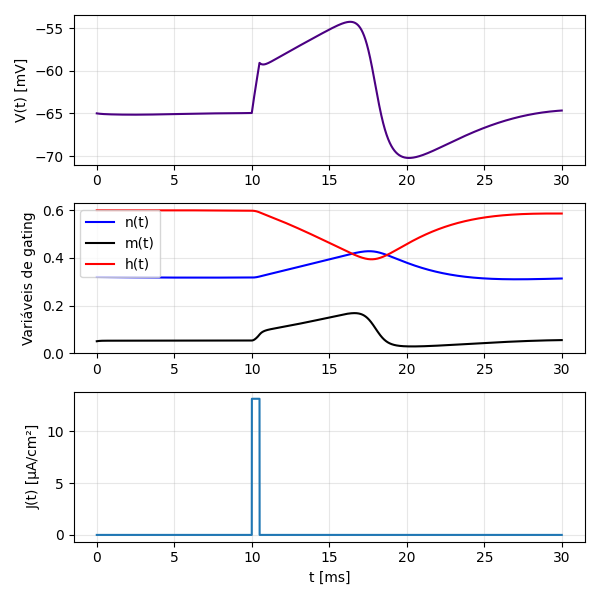
\includegraphics[width=\linewidth]{../figures/ex_2_1.png}
			\captionsetup{justification=centering, labelformat=empty}
			\text{$J = 13,118 \; \mu$A/cm$^2$}
			\label{fig:fig21}
		\end{minipage}
		\hfill
		% Segunda figura
		\begin{minipage}{0.49\textwidth}
			\centering
			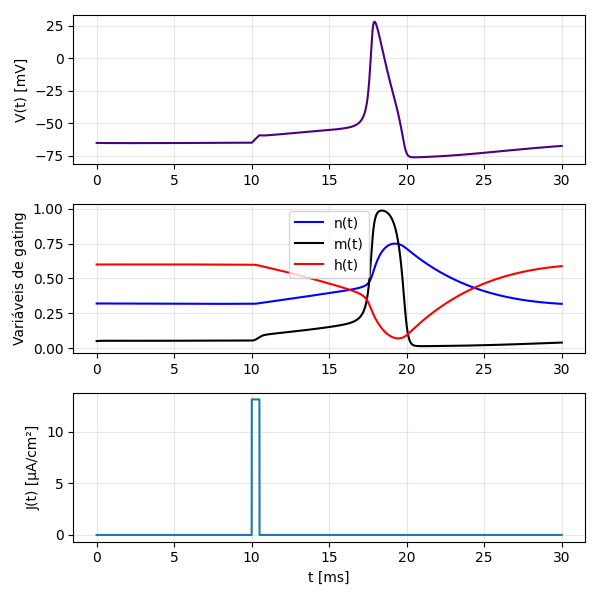
\includegraphics[width=\linewidth]{../figures/ex_2_2.png}
			\captionsetup{justification=centering, labelformat=empty}
			\text{$J = 13,119 \; \mu$A/cm$^2$}
			\label{fig:fig22}
		\end{minipage}
		\caption{Gráficos da simulação para $J$ maior e menor que o limiar de disparo para um pulso de $0,5$ ms.}
		\label{fig2}
	\end{figure}
	
	Assim, o limiar de $J$ para provocar um potencial de ação é aproximadamente $13,119$ $\mu$A/cm$^2$ para os parâmetros do modelo utilizados.\\\\
	
	\noindent \textbf{Questão 3.} Repita o que foi feito na Questão 2, mas agora para pulsos curtos com duração de 1 ms. Como o menor valor estimado de $J$ capaz de provocar um disparo neste caso se compara com o menor valor de $J$ estimado na questão anterior?\\\\
	
	\noindent\textbf{Resposta:} Os gráficos para os dois valores de $J$ do menor intervalo de precisão alcançado estão exibidos na figura \ref{fig3}.
	
	\begin{figure}[H]
		\centering
		% Primeira figura
		\begin{minipage}{0.49\textwidth}
			\centering
			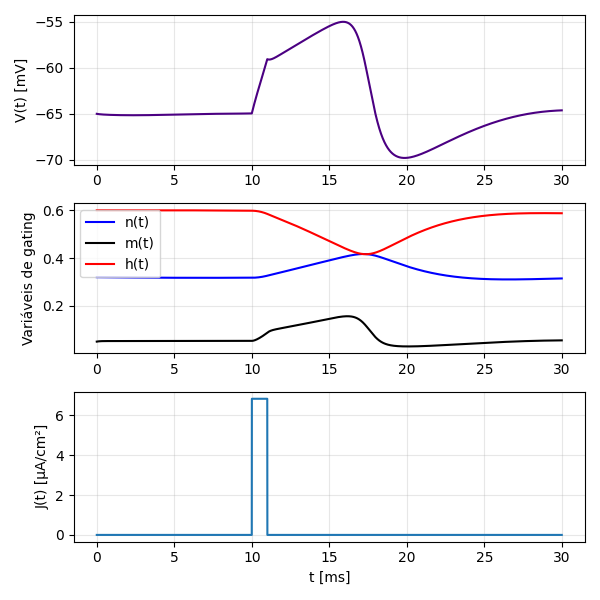
\includegraphics[width=\linewidth]{../figures/ex_3_1.png}
			\captionsetup{justification=centering, labelformat=empty}
			\text{$J = 6,838 \; \mu$A/cm$^2$}
			\label{}
		\end{minipage}
		\hfill
		% Segunda figura
		\begin{minipage}{0.49\textwidth}
			\centering
			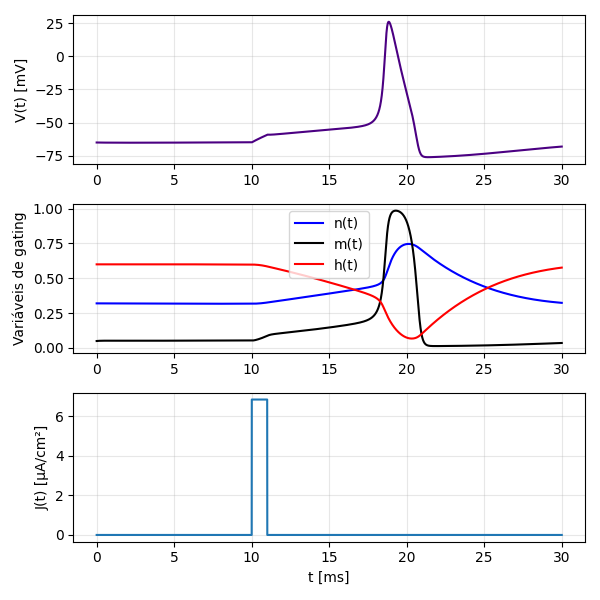
\includegraphics[width=\linewidth]{../figures/ex_3_2.png}
			\captionsetup{justification=centering, labelformat=empty}
			\text{$J = 6,839 \; \mu$A/cm$^2$}
			\label{}
		\end{minipage}
		\caption{Gráficos da simulação para $J$ maior e menor que o limiar de disparo para um pulso de $1$ ms.}
		\label{fig3}
	\end{figure}
	
	Assim, o limiar de $J$ para provocar um potencial de ação é aproximadamente $6,839$ $\mu$A/cm$^2$ quando o pulso tem duração de $1$ ms. Portanto, a intensidade de corrente injetada necessária para causar um disparo é menor quando o disparo tem maior duração. É como se o neurônio tivesse mais tempo para atingir o ponto de efeito cascata onde não há mais retorno.\\\\
	

	
	
	\noindent \textbf{Questão 4.} Use agora o seu programa para simular a resposta do modelo a degraus de densidade de corrente injetada com amplitude $J$. Faça sua simulação durar de 0 a 500 ms e inicie o degrau de densidade de corrente em $t_i = 50$ ms e termine-o em $t_f = 450$ ms. Antes e depois do degrau de densidade de corrente o valor de $J$ deve ser zero. Para esta questão, use como passo de integração para o método de Euler o valor $\Delta t = 0{,}025$ ms. Tente encontrar o menor valor de $J$ capaz de produzir um disparo. Define-se a \textit{reobase} como a menor corrente de duração infinita capaz de provocar um disparo em um neurônio (\url{https://en.wikipedia.org/wiki/Rheobase}). Portanto, o seu estudo resultará em uma aproximação para a reobase do modelo de Hodgkin-Huxley (medida em termos de densidade de corrente). Para isso, use uma estratégia similar à indicada na questão anterior, mas agora comece com $J$ indo de 1 a 20 (em unidades de $\mu$A/cm$^2$) em incrementos de 5 em 5. Depois de determinar a reobase (em unidades de densidade de corrente), tente encontrar a densidade de corrente $J$ que produz dois disparos. Em seguida, tente determinar a densidade de corrente $J$ que produz um trem de disparos enquanto durar a simulação. Entregue seus gráficos para quatro casos: (i) um valor de $J$ que não produz disparos; (ii) o valor de $J$ da reobase; (iii) o valor de $J$ que produz dois disparos; e (iv) o menor valor de $J$ capaz de produzir um trem de disparos pela duração da simulação.\\\\
	
	\noindent\textbf{Resposta:} Na figura \ref{fig4} estão os resultados pedidos para o pulso de duração muito grande.
	
			\begin{figure}[H]
		\centering
		% Primeira figura
		\begin{minipage}{0.49\textwidth}
			\centering
			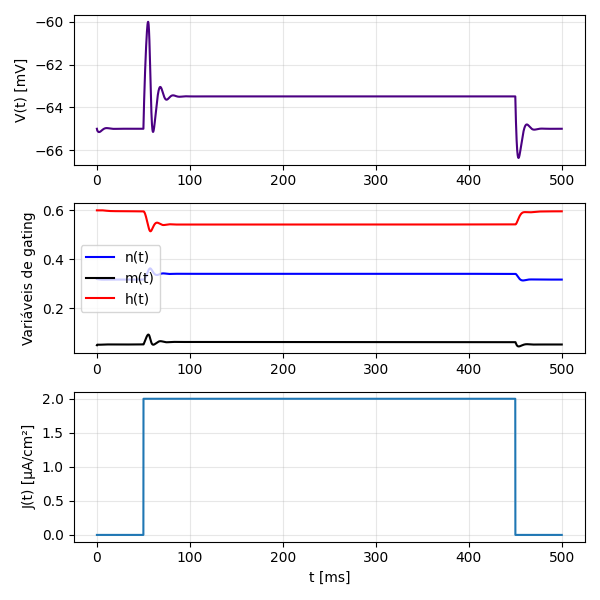
\includegraphics[width=\linewidth]{../figures/ex_4_1.png}
			\captionsetup{justification=centering, labelformat=empty}
			\text{$J = 2,000 \; \mu$A/cm$^2$}
			\label{}
		\end{minipage}
		\hfill
		% Segunda figura
		\begin{minipage}{0.49\textwidth}
			\centering
			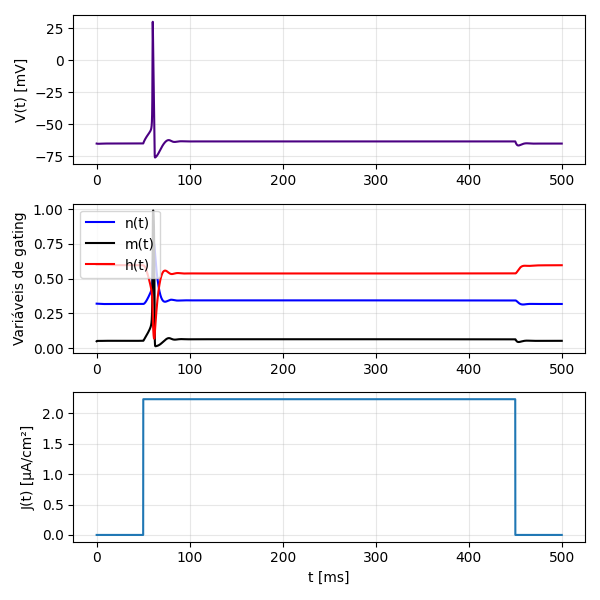
\includegraphics[width=\linewidth]{../figures/ex_4_2.png}
			\captionsetup{justification=centering, labelformat=empty}
			\text{$J = 2,231 \; \mu$A/cm$^2$ (reobase)}
			\label{}
		\end{minipage}
		% Terceira figura
		\begin{minipage}{0.49\textwidth}
			\centering
			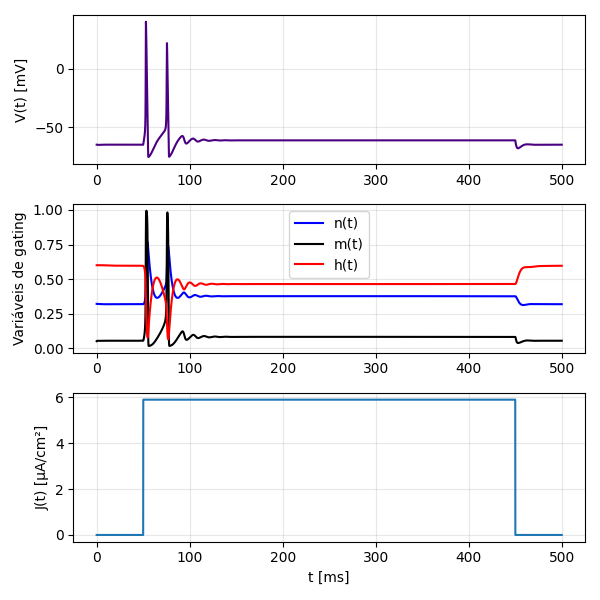
\includegraphics[width=\linewidth]{../figures/ex_4_3.png}
			\captionsetup{justification=centering, labelformat=empty}
			\text{$J = 5,900 \; \mu$A/cm$^2$}
			\label{}
		\end{minipage}
		% Quarta figura
		\begin{minipage}{0.49\textwidth}
			\centering
			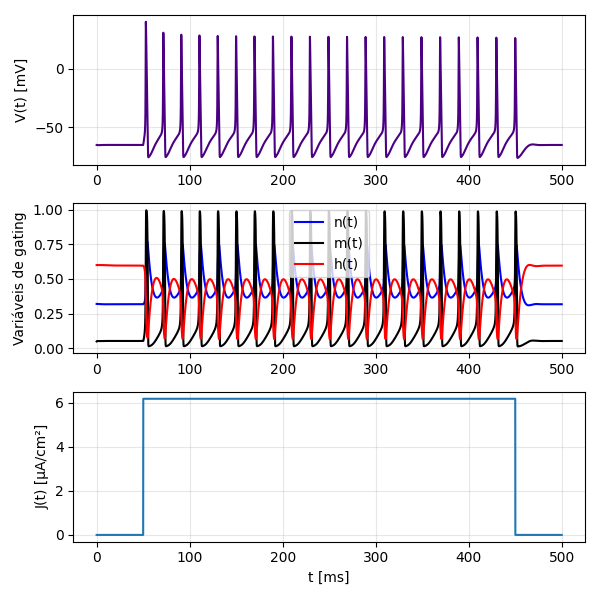
\includegraphics[width=\linewidth]{../figures/ex_4_4.png}
			\captionsetup{justification=centering, labelformat=empty}
			\text{$J = 6,183 \; \mu$A/cm$^2$}
			\label{}
		\end{minipage}
		\caption{Gráficos da simulação para pulso de duração muito grande para os valores de $J$ limiar das condições pedidas na Questão 4.}
		\label{fig4}
	\end{figure}
	
	\noindent \textbf{Questão 5.} Repita a simulação da questão anterior (com $\Delta t = 0{,}025$ ms) para densidades de corrente acima do menor valor encontrado por você para gerar um trem de disparos e construa a curva f-J (frequência \textit{versus} densidade de corrente) do modelo de Hodgkin-Huxley. Tome cuidado na hora de construir a curva f-J, pois a frequência deve estar em hertz (Hz) e o tempo usado nas simulações está em milissegundos. Descreva e justifique o critério usado por você para determinar a frequência de disparos do modelo para cada valor de $J$. Qual é a frequência mínima do trem de disparos? Existe uma frequência máxima? Caso exista, qual é ela? Entregue o gráfico de curva f-J para o modelo de Hodgkin-Huxley. Você consegue explicar por que não ocorrem disparos repetidos com frequências acima da frequência máxima?\\\\
	
	\textbf{Resposta:} A figura \ref{fig5} mostra a curva f-J pedida.
	
	\begin{figure}[H]
		\centering
		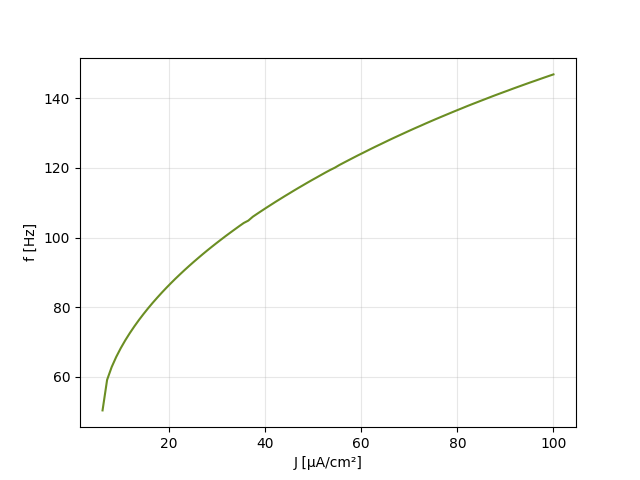
\includegraphics[width=8.5cm]{../figures/ex_5.png}
		\caption{Curva f-J para o modelo HH com os parâmetros dados.}
		\label{fig5}
	\end{figure}
	
	A frequência mínima do trem de disparos é aproximadamente $50,4$ Hz. A frequência máxima é uma questão complexa. Para valores de $J$ grandes, a magnitude dos picos de potencial de ação começam a diminuir, até que, gradualmente, para $J$ suficientemente grande, eles somem. Fica então uma dose de arbitrariedade definir quando podemos considerar que temos um trem de disparos e quando não temos. Por exemplo, quando a magnitude dos disparos não chegam nem a $-50$ mV, podemos chama-los de potenciais de ação efetivamente? Assim, para confeccionar o gráfico da figura \ref{fig5}, escolheu-se arbitrariamente um valor mínimo de magnitude de disparo para o qual medir a frequência, no caso $-30$ mV. Contando quantas vezes a curva cortava a linha dos $-30$ mV e em quanto tempo, foi possível calcular a frequência dividindo a quantidade de cruzamentos pelo tempo tomado (com as devidas correções de unidades). Esta última conta foi feita para 100 valores de $J$ entre $6,183$ $\mu$A/cm$^2$ e $100$ $\mu$A/cm$^2$.
	
	Para os valores de $J$ suficientemente grandes em que o trem esvanece, entende-se que os disparos ficam tão próximos um do outro que eles começam a invadir o período refratário absoluto do disparo anterior, anulando a si mesmos.\\\\
	
	
	\noindent \textbf{Questão 6.} Nesta questão você estudará o período refratário do modelo de Hodgkin-Huxley. Considere novamente um pulso de corrente com duração de 0,5 ms como na Questão 2 e use como $J$ um valor escolhido por você maior que o estimado naquela questão, de maneira que você tenha certeza que o pulso de amplitude $J$ produz um potencial de ação. Vamos chamar este pulso de $J_1$. Altere o seu programa para que agora ele simule a aplicação de dois pulsos de corrente com duração de 0,5 ms: o primeiro com a amplitude $J_1$ aplicado em $t_1 = 10$ ms e o segundo com amplitude $J_2$ aplicado em $t_2 = t_1 + L$, onde $L > 0$ é a latência do segundo pulso em relação ao primeiro. Faça a sua simulação rodar por um tempo maior que 30 ms (entre 80 e 100 ms deve ser suficiente) e volte a usar como passo de tempo para o método de Euler o valor $\Delta t = 0{,}001$ ms. Inicialmente, faça $J_2 = J_1$ e tente encontrar o menor valor de $L$ tal que o segundo pulso produza um potencial de ação. Este é o período refratário relativo do modelo para o pulso utilizado. Em seguida, repita o que foi feito para alguns valores de $J_2$ maiores que $J_1$ e tente encontrar o período refratário absoluto do modelo. Nesse estudo, pode ser útil construir um gráfico da latência $L$ \textit{versus} a amplitude $J_2$ do segundo estímulo. Tome cuidado, pois nem tudo que se parece com um potencial de ação é de fato um potencial de ação. Para determinar se a resposta do neurônio é um potencial de ação, observe o comportamento do crescimento da amplitude do pulso de voltagem em função de $J_2$. Enquanto esse crescimento for aproximadamente linear, não existe um potencial de ação.\\\\
	
	\noindent\textbf{Resposta:} Para $J_1 = J_2 = 15$ $\mu$A/cm$^2$, obteve-se $L = 16,74$ ms como latência mínima para produzir o segundo potencial de ação. O gráfico deste resultado pode ser visto na figura \ref{fig6}.
	
	\begin{figure}[H]
		\centering
		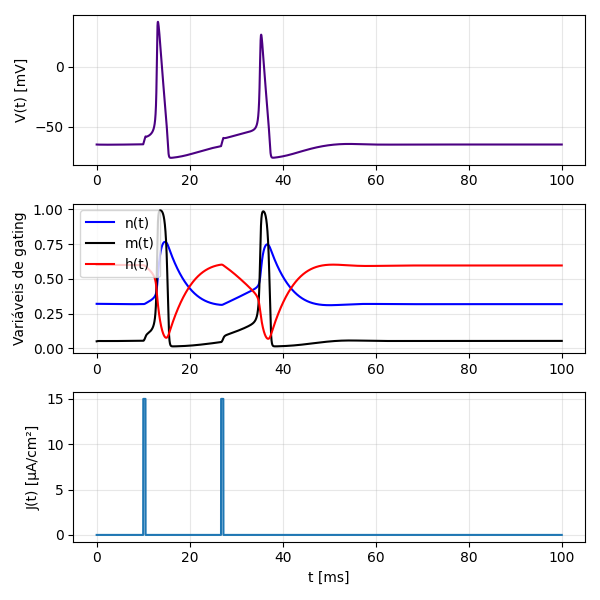
\includegraphics[width=8.5cm]{../figures/ex_6_1.png}
		\caption{Curvas de dois disparos causados por corrente de mesma intensidade com latência mínima entre eles.}
		\label{fig6}
	\end{figure}
	
	Na figura \ref{fig7} temos o gráfico de $L$ \textit{versus} $J$.
	
		\begin{figure}[H]
		\centering
		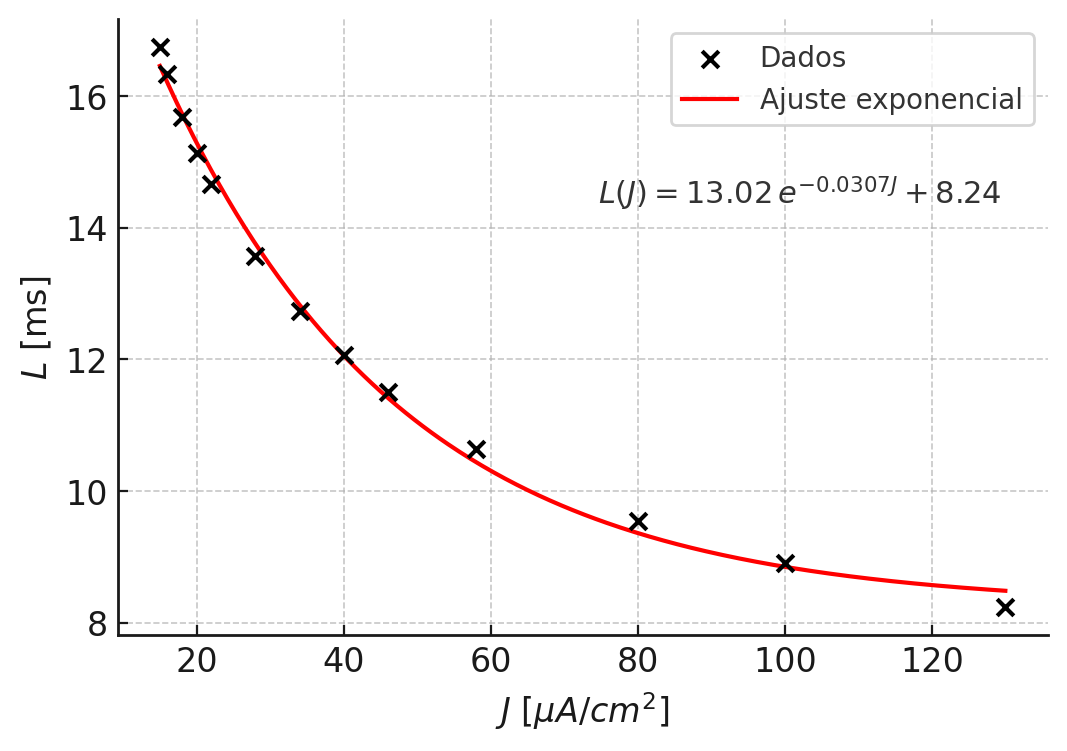
\includegraphics[width=8.5cm]{../figures/ex_6_2.png}
		\caption{Curvas de $L$ em função de $J$ com \textit{fitting} exponencial.}
		\label{fig7}
	\end{figure}
	
	A curva foi ajustada para uma função exponencial (escrita na figura). Com $J \rightarrow \infty$, $L$ tende a $8,24$ ms na curva ajustada. Isso quer dizer que, não importa quão grande $J$ seja, a latência do segundo disparo nunca vai ser menor que a assíntota $L = 8,24$ ms. Mas isto é exatamente o que definimos como o período refratário absoluto, no qual é impossível haver um segundo disparo. Logo, o período refratário absoluto desta simulação é de $8,24$ ms.\\\\
	
	
	\noindent \textbf{Questão 7.} Simule agora a resposta do modelo a uma corrente hiperpolarizante, isto é, negativa e tente observar o fenômeno de estimulação de quebra de anodo. Ao contrário das questões anteriores, faça agora a densidade de corrente injetada ser constante e igual a $J = -15$ $\mu$A/cm$^2$ e varie o intervalo pelo qual ela é aplicada. Faça a simulação total durar de $t = 0$ a $t = 30$ ms com o degrau de corrente indo de $t_i = 5$ ms a $t_f = t_i + T$ com $T$ variável. Use valores de $T$ (em ms) indo de 0,5 a 5,0 em incrementos de 0,5. Use como passo de tempo para o método de Euler o valor $\Delta t = 0{,}001$ ms. Qual o menor valor de $T$ para o qual um potencial de ação é gerado após o desligamento da corrente hiperpolarizante? E qual o atraso entre o instante do término da corrente e o instante do início do potencial de ação? Considere que o potencial de ação se inicia quando $V \geq 20$ mV. Entregue gráficos para dois valores diferentes de $T$: um para o qual não ocorre um potencial de ação e outro para o qual ocorre um potencial de ação.\\\\
	
	\noindent\textbf{Resposta:} Para incrementos feitos ao modo do enunciado, o menor valor de $T$ encontrado para gerar um potencial de ação foi $1,5$ ms. A figura \ref{fig8} mostra os gráficos para $T = 1$ ms (não gera disparo) e para $T =  1,5$ ms (gera disparo).
	
		\begin{figure}[H]
		\centering
		% Primeira figura
		\begin{minipage}{0.49\textwidth}
			\centering
			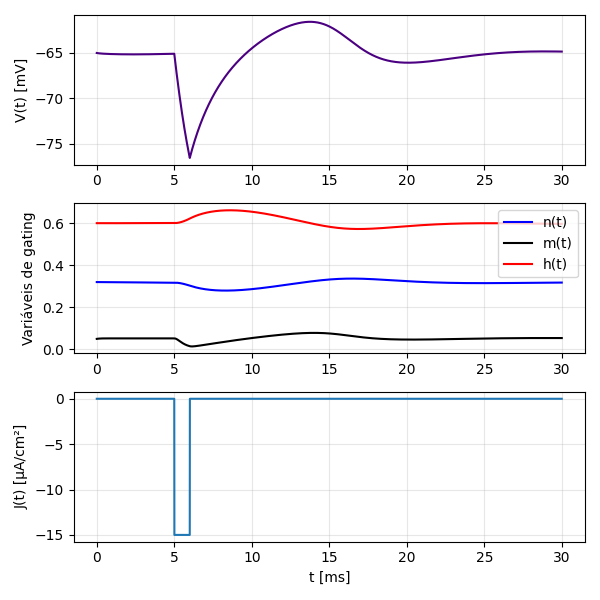
\includegraphics[width=\linewidth]{../figures/ex_7_1.png}
			\captionsetup{justification=centering, labelformat=empty}
			\text{$T = 1$ ms}
			\label{}
		\end{minipage}
		\hfill
		% Segunda figura
		\begin{minipage}{0.49\textwidth}
			\centering
			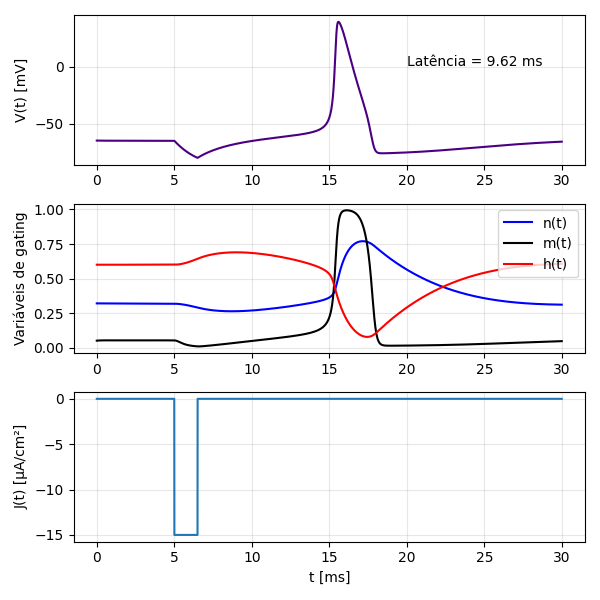
\includegraphics[width=\linewidth]{../figures/ex_7_2.png}
			\captionsetup{justification=centering, labelformat=empty}
			\text{$T = 1,5$ ms}
			\label{}
		\end{minipage}
		\caption{Gráficos do efeito de corrente hiperpolarizante de durações diferentes.}
		\label{fig8}
	\end{figure}
	
	Para $T = 1,5$ ms, o tempo decorrido entre o desligamento da corrente hiperpolarizante até o início do potencial de ação foi de $9,62$ ms (também escrito na figura).
	
	
	
	
	
	
\end{document}